% =============================================================================
% thesis-split.tex
% 修士論文（分割粒度に焦点を絞った版）
%
% スポットインスタンス上の短時間ワークロードにおける
% 分割粒度を考慮した中断対策
%
% 構成:
%   第1章 序論
%   第2章 関連研究
%   第3章 中断特性の実測          <- main.tex (背景・枠組み・実験設定) を活用
%   第4章 分割粒度を考慮した実行モデル
%   第5章 検証計画
%   第6章 結論
%
% コンパイル: lualatex thesis-split.tex (2回)
% =============================================================================
\documentclass[11pt,a4paper]{ltjsreport}

\usepackage{luatexja}
\usepackage{amsmath,amssymb}
\usepackage{graphicx}
\usepackage{booktabs}
\usepackage{tabularx}
\usepackage{array}
\usepackage{geometry}
\usepackage{caption}
\usepackage{url}
\usepackage[hidelinks]{hyperref}

\geometry{top=30mm,bottom=30mm,left=28mm,right=28mm}
\captionsetup[figure]{labelsep=quad,font=small}
\captionsetup[table]{labelsep=quad,font=small}

\newcommand{\Fcomp}{F_{\mathrm{comp}}}
\newcommand{\Rlaunch}{R_{\mathrm{launch}}}
\newcommand{\Rint}{R_{\mathrm{int}}}
\newcommand{\Nreq}{N_{\mathrm{req}}}
\newcommand{\Nsucc}{N_{\mathrm{succ}}}
\newcommand{\Nint}{N_{\mathrm{int}}}
\newcommand{\E}{\mathbb{E}}
\newcommand{\Waste}{\mathrm{Waste}}

\title{\vspace{-10mm}
スポットインスタンス上の短時間ワークロードにおける\\
分割粒度を考慮した中断対策}
\author{那須 渚}
\date{2026年度 修士論文\\[2mm] 同志社大学大学院 理工学研究科}

\begin{document}
\maketitle

% =============================================================================
\chapter*{概要}
\addcontentsline{toc}{chapter}{概要}

スポットインスタンスはクラウド利用コストを大幅に削減できる一方，
提供側の都合により中断される可能性がある．
CI/CD のビルドやテストのような短時間ワークロードでは，
中断が発生するとジョブ全体の再実行が必要となり，
実行時間と利用コストの双方が増加する．

本論文は，\textbf{中断によって失われる時間をどう減らすか}という問いに取り組む．
スポットインスタンスには中断の約 2 分前に警告が通知される機構があり，
これを利用できるならば事前の備えは不要である．
そこで本論文は，中断への備え方を
\textbf{あらかじめ分割しておく方式}と
\textbf{警告を受けてから対処する方式}の二つに整理し，
どちらを採用すべきかの境界と，
分割を選ぶ場合の粒度の決定法を与える．

まず，短時間ワークロードにおけるスポットインスタンスの信頼性を，
起動可能性ではなく\textbf{期限条件付き完了可能性} $\Fcomp(d)$ として
定義する測定フレームワークを構築した．
AWS の 4 リージョン・3 インスタンスタイプを対象に
1 週間（$\Nreq = 2{,}016$）の実測を行い，
起動成功率 $96.7\%$，中断率 $6.0\%$ を観測した．

この実測データの分析により，中断ハザード率が経過時間によらず
ほぼ一定（0.054--0.130 \%/分）であり，
中断が近似的にメモリレスな事象として振る舞うことを示した．
この性質のもとでは，ジョブを $k$ 個の断片に分割し
チェックポイントで接続することにより，
断片あたりの被中断確率と中断時の損失量が同時に低下する．

ただし，中断は大部分の実行では発生しない（観測された中断率は $6.0\%$）．
したがって，中断時にのみコストを支払う警告駆動復旧が有利となりうる．
その成立条件を，猶予時間内に保存と復旧が完了すること（$c + s < 120$ 秒），
任意の時点で一貫した状態を保存できること，
警告が十分な確率で通知されることの三点として定式化した．
条件を満たす場合，警告駆動復旧の無駄時間は $0.1$ 分未満にとどまり，
\textbf{事前の分割は不要である}．

一方これらを満たさない場合には事前分割が必要となる．
分割には起動およびチェックポイントのコストが伴うため，
総無駄時間は分割数に対して U 字型となり，
\textbf{最適分割数 $k^{*}$ が存在する}ことが示された．
「細かく分割するほどよい」という直観は成立しない．

さらに感度分析により，$k^{*}$ がチェックポイントコスト $c$ に
極めて敏感であることを明らかにした．
$c = 0$ では $k^{*} = 6$ であるが，$c = 5$ 秒で $k^{*} = 2$ に低下し，
$c \geq 60$ 秒では分割そのものが無効となる．
$c$ が大きい領域では警告駆動復旧と事前分割がともに成立せず，
実行条件の選択に頼るほかない．

$c$ はワークロードの性質に依存する未実測量である．
以上を踏まえ，$c$ の実測を最優先とする検証計画を提示する．

% =============================================================================
\tableofcontents
\listoffigures
\listoftables

% =============================================================================
\chapter{序論}

\section{研究背景}

近年，クラウドコンピューティングは企業，研究機関，個人開発者によって
広く利用されている．
クラウド利用の規模が拡大し，高性能な計算資源への需要が増加するにつれて，
その利用コストは多くの利用者にとって重要な課題となっている．

コストを削減する手法の一つに，スポットインスタンスの利用がある．
スポットインスタンスは，クラウドプロバイダが余剰計算資源を
オンデマンドインスタンスより低価格で提供する料金モデルである~\cite{AWSSpot}．
オンデマンドインスタンスと比較して，
数十パーセントから最大約 90\% の割引価格で利用できる~\cite{Lin2022Survey}．
そのため，機械学習やバッチ処理のような大規模計算ワークロードだけでなく，
CI/CD における自動ビルドやテストのように
一時的に計算資源を必要とするワークロードにも利用されている~\cite{Ramesh2025}．

しかしスポットインスタンスは余剰容量に基づいて提供されるため，
クラウド需要が増加した場合や利用可能容量が減少した場合に中断されうる．
この中断を interruption event と呼ぶ．
ワークロードの実行中に interruption event が発生すると，
実行中の処理が完了前に停止する．
特にバッチ処理，機械学習，CI/CD のビルドやテストが中断された場合，
ワークロード全体の再実行が必要となり，
実行時間と利用コストの双方が増加する．

\section{問題意識}

既存のアプローチとしては，価格変動を考慮した入札戦略や，
Spot Placement Score（SPS）のようなプロバイダ固有の
可用性指標に基づく選択が挙げられる~\cite{Garg2025,Katayama2022}．
SPS は，スポットリクエストが成立する可能性を推定する上で有用である．

しかし，CI/CD パイプラインやバッチ処理ジョブのような
短時間ワークロードの利用者にとって，より実用的な問いは
\textbf{スポットインスタンスを起動できるかどうか}だけではなく，
\textbf{ワークロードが完了するまで利用し続けられるかどうか}である．

起動に成功したとしても，ワークロード完了前に中断されれば，
短時間ワークロードは失敗する．
すなわち\textbf{起動時点の可用性}と\textbf{起動後の継続性}は
異なる問題であり，既存指標は前者のみを扱っている．

\section{本研究の問い}
\label{sec:question}

本論文を貫く問いは一つである．

\begin{quote}
\textbf{中断によって失われる時間を最小化するには，
ジョブをどのような単位で実行すればよいか．}
\end{quote}

この問いに答えるには，まず「失われる時間」を定量化する必要がある．

中断されるとジョブは再実行される．
したがって利用者が支払う総時間は，
本来必要な計算時間に加え，
中断された試行で費やされた時間が上乗せされる．
この上乗せ分を\textbf{無駄時間}と呼び，本論文の最小化対象とする．

無駄時間は二つの要素の積として近似できる．

\begin{equation}
\text{無駄時間} \;\approx\;
\underbrace{\text{やり直す回数}}_{\text{中断されにくさで決まる}}
\;\times\;
\underbrace{\text{1 回あたりの損失}}_{\text{1 回の実行の長さで決まる}}
\label{eq:intro_waste}
\end{equation}

ここで注目すべきは，\textbf{両要素がいずれも
「1 回の実行をどれだけの長さにするか」に依存する}点である．

実行単位を短くすれば，その実行が中断に遭遇する確率は下がる（第一要素）．
同時に，中断された場合に失われる時間も短くなる（第二要素）．
したがって，ジョブを $k$ 個の断片に分割し，
チェックポイントによって接続すれば，
二つの要素を同時に削減できる可能性がある．

一方で，分割は無償ではない．
断片ごとにインスタンスの起動コストと
チェックポイントの保存・復元コストが発生するため，
分割しすぎればかえって総時間が増加する．

ただし実際のスポットインスタンスには，
中断の約 2 分前に警告が通知される機構が存在する．
この警告を利用できるならば，事前に分割しておく必要はなく，
\textbf{警告を受けた時点で状態を保存すればよい}．
中断は大部分の実行では発生しないため，
平常時のコストを支払わないこの方式には本質的な利点がある．

したがって中断への備え方には，
\textbf{あらかじめ分割しておく}方式と，
\textbf{警告を受けてから対処する}方式の二つがある．
両者はコストの支払い方が異なり，
どちらが有利かは中断の発生頻度，チェックポイントのコスト，
および警告の信頼性に依存する．

本論文の問いは，いずれか一方の優劣を論じることではなく，
次の二段階の判断を定量的に与えることである．

\begin{enumerate}
  \item \textbf{どちらの備え方を採用すべきか}．
        その境界はどこにあるか．
  \item 事前分割を選ぶ場合，\textbf{どの粒度で分割すべきか}．
\end{enumerate}

この問いの立て方により，
警告が十分に機能する環境では「事前の分割は不要である」という結論が，
機能しない環境では「分割が必要であり，その粒度は $k^{*}$ である」
という結論が，\textbf{いずれも同一の枠組みから導かれる}．

\section{本論文のアプローチ}

提案手法を設計するには，まず対象環境における
中断の実測データが必要である．
式~\eqref{eq:intro_waste} の二要素は，いずれも
「どの程度の長さの実行が，どの程度中断されるか」という
実測値に基づいて初めて定量化できるためである．

そこで本論文は次の順序で進める．

\begin{enumerate}
  \item \textbf{実測}（第~\ref{chap:measure} 章）：
        スポットインスタンスの信頼性を
        期限条件付き完了可能性 $\Fcomp(d)$ として定義し，
        測定フレームワークを実装して実測データを取得する．
  \item \textbf{モデル化}（第~\ref{chap:split} 章）：
        実測データから中断のメモリレス性を確認し，
        分割粒度 $k$ を決定変数とするコストモデルを構築する．
  \item \textbf{検証計画}（第~\ref{chap:plan} 章）：
        モデルの未確定要素を同定し，
        それを解消する実験計画を示す．
\end{enumerate}

\section{本論文の貢献}

本論文の貢献は以下の通りである．

\begin{enumerate}
  \item 短時間ワークロードにおけるスポットインスタンスの信頼性を，
        起動可能性やインフラレベルの生存時間ではなく，
        \textbf{期限条件付き完了可能性} $\Fcomp(d)$ として定義し，
        起動成功と起動後の中断挙動を分離して記録する
        測定フレームワークを実装した（第~\ref{chap:measure} 章）．
  \item 4 リージョン・3 インスタンスタイプ・1 週間の実測により，
        \textbf{中断ハザード率が経過時間によらずほぼ一定}であること，
        すなわち中断が近似的にメモリレスな事象として振る舞うことを示した
        （第~\ref{chap:measure} 章）．
  \item 中断への二つの備え方（事前分割と警告駆動復旧）を
        同一のコストモデル上で比較し，
        \textbf{いずれを採用すべきかを決定する枠組み}を与えた．
        境界は三条件，すなわち猶予時間内に保存と復旧が完了すること
        （$c + s < 120$ 秒），任意の時点で保存できること，
        警告が十分な確率で通知されることにより定まる
        （第~\ref{chap:split} 章）．
  \item 枠組みの帰結として，
        \textbf{条件を満たす環境では定期的なチェックポイント取得は不要であり，
        かえって無駄時間を増加させる}ことを定量的に示した．
        広く行われている慣行が必ずしも最適でないことを意味する
        （第~\ref{chap:split} 章）．
  \item 条件を満たさない場合の手段として
        \textbf{分割粒度 $k$ を設計変数とするコストモデル}を構築し，
        総無駄時間が $k$ に対して U 字型となること，
        すなわち\textbf{最適分割数 $k^{*}$ が存在する}ことを
        定量的に示した（第~\ref{chap:split} 章）．
  \item $k^{*}$ が\textbf{チェックポイントコストに支配される}ことを
        感度分析により明らかにし，
        $c$ の大きさに応じた対策の選択指針を提示した
        （第~\ref{chap:split} 章）．
  \item モデルの未確定要素を同定し，
        それを最短で解消する検証計画を設計した
        （第~\ref{chap:plan} 章）．
\end{enumerate}

\section{本論文の構成}

第~\ref{chap:related} 章では関連研究を整理する．
第~\ref{chap:measure} 章では測定フレームワークと実測結果を示し，
中断のメモリレス性を明らかにする．
第~\ref{chap:split} 章では分割粒度を決定変数とするモデルを提案する．
第~\ref{chap:plan} 章では検証計画を述べる．
第~\ref{chap:conclusion} 章で本論文をまとめる．

% =============================================================================
\chapter{関連研究}
\label{chap:related}

\section{スポットインスタンスの可用性と中断対策}

スポットインスタンスの可用性および信頼性については，
これまでに複数の研究が行われている．
Lin ら~\cite{Lin2022Survey} は可用性を向上させる手法を調査し，
チェックポイント，マイグレーション，レプリケーション，スケジューリング
といったアプローチを整理している．
これらの研究は，スポットインスタンスを実用的に利用するうえで
中断リスクが中心的課題であることを示している．

SPS は AWS が提供するプロバイダ固有の指標であり，
インスタンスタイプ，リージョン，必要容量などの条件下で
スポットリクエストが成立する可能性を推定するために用いられる~\cite{AWSSPS}．
Katayama ら~\cite{Katayama2022} はマイグレーション先の選択に SPS を用い，
起動時点の可用性を向上させられることを示した．

ただし SPS は，起動に成功したインスタンスが
ワークロードを完了するのに十分な時間
利用可能な状態を維持できるかどうかを直接示すものではない．

\section{中断挙動の時間的特性}

Kim ら~\cite{Kim2024SpotInterruption} は，
SPS が時間帯や曜日に応じて周期的に変動し，
survival time と一定の関係を持つことを示している．
Lee ら~\cite{Lee2022SpotLake} は，SPS，スポット価格，中断率などを
継続的に収集・保存するアーカイブサービス SpotLake を提案し，
GPU インスタンスや大規模インスタンスタイプで
可用性が低くなる傾向があることを報告している．

これらの研究は中断挙動の統計的性質を明らかにしているが，
その焦点はインフラレベルの可用性データの収集と分析にある．
\textbf{中断がどのような時間的分布で発生するか}，
とりわけ\textbf{経過時間に対するハザード率の挙動}が
ワークロードの実行単位の設計に与える含意については，
十分に検討されていない．

\section{チェックポイントと分割実行}

中断対策としてのチェックポイントは古くから研究されている~\cite{Lin2022Survey}．
機械学習の分野ではエポック単位でのモデル保存が一般的であり，
CI/CD の分野でもテストのシャード分割やビルドキャッシュといった形で
事実上の分割実行が広く行われている．

ただし既存研究および実務の多くは，チェックポイントを
「中断に備えて取るもの」として定性的に扱っている．
チェックポイントの間隔は，実装の都合や
処理の自然な区切り（エポック，テストスイート単位）によって
決められることが多い．

これに対し本研究は，\textbf{分割粒度そのものを最適化対象}とし，
その最適値が中断特性とチェックポイントコストによって
定量的に決定されることを示す点で異なる．

\section{本研究の位置づけ}

既存研究に対する本研究の位置づけを表~\ref{tab:related} に示す．

\begin{table}[htbp]
\centering
\caption{関連研究と本研究の位置づけ}
\label{tab:related}
\small
\begin{tabularx}{\textwidth}{@{}lXX@{}}
\toprule
 & \textbf{着目する側面} & \textbf{設計変数} \\
\midrule
SPS~\cite{AWSSPS}，Katayama ら~\cite{Katayama2022}
  & 起動時点の可用性
  & リージョン，AZ \\
\addlinespace
Kim ら~\cite{Kim2024SpotInterruption}，
Lee ら~\cite{Lee2022SpotLake}
  & 中断挙動の統計的性質
  & （分析対象であり設計変数ではない） \\
\addlinespace
従来のチェックポイント手法~\cite{Lin2022Survey}
  & 中断からの復旧
  & （実装都合で決める。最適化対象ではない） \\
\addlinespace
\textbf{本研究}
  & \textbf{期限条件付き完了可能性}
  & \textbf{分割粒度 $k$} \\
\bottomrule
\end{tabularx}
\end{table}

% =============================================================================
\chapter{中断特性の実測}
\label{chap:measure}

\section{本章のねらい}

第~\ref{chap:split} 章で構築するコストモデルは，
式~\eqref{eq:intro_waste} の二要素を定量化した値を入力として要求する．
具体的には次の三つである．

\begin{itemize}
  \item 長さ $T$ の実行が中断されずに完了する確率
  \item 中断された場合に失われる時間の期待値
  \item インスタンスの起動オーバーヘッド
\end{itemize}

これらはいずれも対象環境における実測値であり，
文献値では代用できない．
本章では，これらを取得するための測定フレームワークを構築し，
AWS 上で実測を行う．

さらに，取得したデータから\textbf{中断ハザード率の挙動}を分析する．
これは第~\ref{chap:split} 章の提案が成立するための前提条件となる．

\section{期限条件付き完了可能性}

\subsection{問題の定義}

SPS のような既存指標は，スポットリクエストが成立するかどうかを特徴づける．
しかし，起動に成功したインスタンスが
ワークロード完了まで利用可能であり続けるかどうかは示さない．

CI/CD パイプラインやバッチジョブのような短時間ワークロードにとって，
この二つは異なる関心事である．
起動に成功しても完了前に中断されれば，ジョブ全体の再実行が必要となり，
実行時間とコストの双方が増加する．
したがって利用者には，リクエスト成立可能性ではなく
\textbf{期限指向のスポット信頼性}が必要である．

\subsection{指標の定義}

本研究では実際のアプリケーションレベルのワークロードは実行しない．
代わりに，指定期限まで中断されずに利用可能であることを
\textbf{ワークロード完了可能性の proxy} として用いる．
すなわち，起動に成功したインスタンスが期限 $d$ より前に
中断されなかった場合，観測条件下において
その実行時間要件を持つ短時間ワークロードは完了可能とみなす．

$\Nreq$ をスポットインスタンスの起動リクエスト数，
$\Nsucc$ を起動に成功したインスタンス数，
$\Nint(d)$ を期限 $d$ より前に中断された
起動成功インスタンス数とする．

\textbf{起動成功率}を次のように定義する．

\begin{equation}
\Rlaunch = \frac{\Nsucc}{\Nreq}
\label{eq:rlaunch}
\end{equation}

\textbf{期限前中断率}を次のように定義する．

\begin{equation}
\Rint(d) = \frac{\Nint(d)}{\Nsucc}
\label{eq:rint}
\end{equation}

さらに\textbf{期限条件付き完了可能性}を次のように定義する．

\begin{equation}
\boxed{\;\Fcomp(d) = 1 - \Rint(d)\;}
\label{eq:fcomp}
\end{equation}

この指標は，起動に成功したインスタンスのうち
期限 $d$ まで利用可能な状態を維持した割合を表す．
ただしこれは実際のアプリケーションレベルの成功率ではなく，
\textbf{インスタンスの生存に基づく proxy} として解釈すべきである．

式~\eqref{eq:rlaunch} と式~\eqref{eq:rint} を分離して定義することにより，
起動時点の容量不足に起因する失敗と，
起動後に発生する中断とを区別して分析できる．

\section{測定フレームワーク}

図~\ref{fig:framework} に測定フレームワークを示す．
本フレームワークでは，スケジューラを用いて
スポットインスタンスの起動リクエストを定期的に送信し，
起動結果，稼働状態，中断状態を収集する．

\begin{figure}[htbp]
\centering
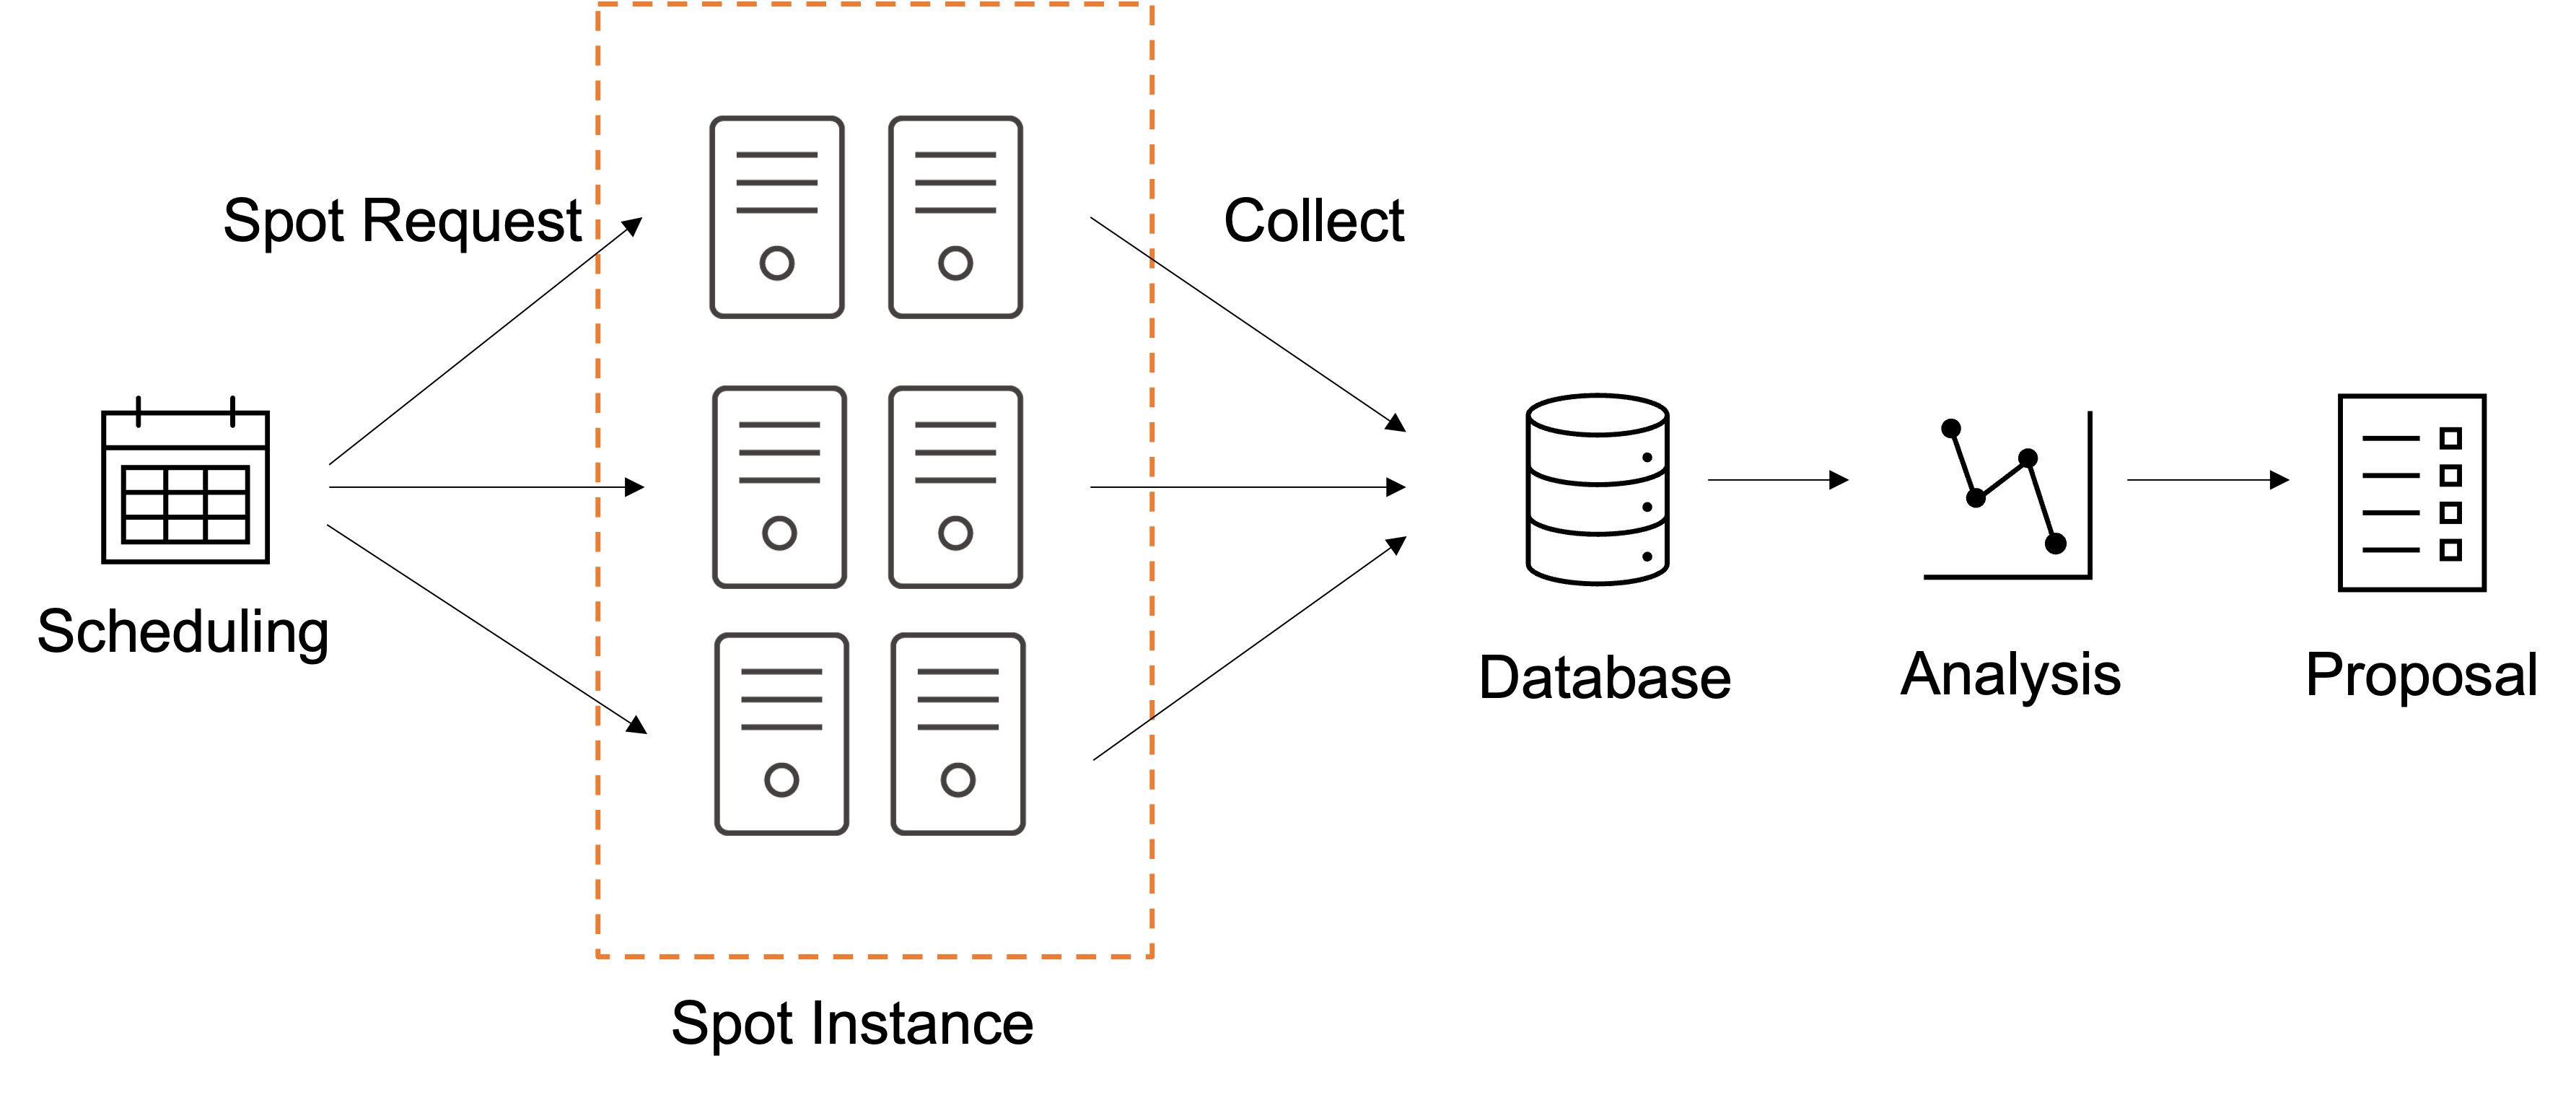
\includegraphics[width=\textwidth]{images/artect.png}
\caption{測定フレームワーク}
\label{fig:framework}
\end{figure}

スケジューラは対象とする各インスタンスタイプに対して
定期的に起動リクエストを送信する．
起動に成功した各インスタンスは 1 時間の固定観測期間にわたって監視される．
この期間中，システムはリクエストが成立したか，
インスタンスがどの程度の時間利用可能であったか，
予定終了時刻より前に interruption event が発生したかを記録する．
観測期間内に中断が発生しなかった場合，
インスタンスはシステムによって終了される．

スポット中断と通常のシステム終了を区別するため，
測定システムによって終了されることなく
予定された 1 時間の観測終了前に利用不能となったインスタンスを
中断候補として扱う．

\section{実験設定}

\paragraph{インスタンスタイプ．}
異なるリソース特性を持つインスタンスタイプ間で中断傾向を比較するため，
3 種類を代表例として選定した~\cite{Pham2018,AWSInstanceTypes}．
仕様を表~\ref{tab:specs} に示す．

\begin{table}[htbp]
\centering
\caption{評価対象インスタンスタイプの仕様。観測スポット価格は観測期間中
（2026年5月19日--25日）に 4 リージョンで記録された平均時間単価（USD/h）である。}
\label{tab:specs}
\small
\begin{tabularx}{\textwidth}{@{}l>{\raggedright\arraybackslash}X>{\raggedright\arraybackslash}X>{\raggedright\arraybackslash}X@{}}
\toprule
 & \textbf{c6a.large} & \textbf{g4dn.xlarge} & \textbf{t3.micro} \\
\midrule
分類 & 計算最適化 & GPU 搭載 & バースト可能汎用 \\
プロセッサ & AMD EPYC (3rd gen) & Intel Xeon (Cascade Lake) & Intel Xeon (burstable) \\
vCPU & 2 & 4 & 2 (burstable) \\
メモリ & 4 GiB & 16 GiB & 1 GiB \\
GPU & --- & 1$\times$ NVIDIA T4 (16 GiB) & --- \\
ローカルストレージ & EBS のみ & 125 GB NVMe SSD & EBS のみ \\
観測スポット価格 & 0.038 & 0.277 & 0.005 \\
\bottomrule
\end{tabularx}
\end{table}

\paragraph{リージョン．}
対象リージョンは N.~Virginia (us-east-1)，Tokyo (ap-northeast-1)，
Ireland (eu-west-1)，Singapore (ap-southeast-1) の 4 つである．
各リージョンにおいて，各インスタンスタイプにつき 1 時間に 1 台を起動する．

\paragraph{時間帯の区分．}
中断傾向が実行タイミングによって異なる可能性を考慮し，
タイムスタンプを各リージョンのローカル時刻に正規化したうえで，
ローカル 1 日を 6 時間ずつの 4 区間に分割して記録する
（表~\ref{tab:periods}）．
この区分は第~\ref{chap:split} 章において，
提案手法の効果が条件によってどう変わるかを分析する際に用いる．

\begin{table}[htbp]
\centering
\caption{ローカル時間帯の区分}
\label{tab:periods}
\small
\begin{tabular}{@{}ll@{}}
\toprule
区分 & ローカル時刻 \\
\midrule
Night     & 00:00--05:59 \\
Morning   & 06:00--11:59 \\
Afternoon & 12:00--17:59 \\
Evening   & 18:00--23:59 \\
\bottomrule
\end{tabular}
\end{table}

\paragraph{観測期間と価格設定．}
実験は 2026 年 5 月 19 日から 5 月 25 日まで実施した．
スポットリクエストでは最大スポット価格を指定していない．
したがって本実験は，AWS のデフォルトのスポット価格設定における
挙動を観測している．

\section{実測結果}

\subsection{全体の傾向}

観測期間中，4 リージョン・3 インスタンスタイプにわたり
合計 $\Nreq = 2{,}016$ 件の起動リクエストを送信した．
このうち $\Nsucc = 1{,}950$ 件が正常に起動し，
全体の起動成功率は $\Rlaunch = 96.7\%$ であった．
起動に成功したインスタンスのうち 117 件（$6.0\%$）が
1 時間の観測期間終了前に中断された．

期限 $d$ ごとの $\Fcomp(d)$ を表~\ref{tab:fcomp_overall} に示す．

\begin{table}[htbp]
\centering
\caption{期限 $d$ ごとの $\Fcomp(d)$（全データをプール，$\Nsucc = 1{,}950$）}
\label{tab:fcomp_overall}
\small
\begin{tabular}{@{}lrrrr@{}}
\toprule
期限 $d$ & 5 分 & 10 分 & 30 分 & 60 分 \\
\midrule
$\Fcomp(d)$ & 0.9938 & 0.9882 & 0.9692 & 0.9451 \\
\bottomrule
\end{tabular}
\end{table}

\textbf{短い期限ほど完了可能性が高い}という傾向が明確に表れている．
この観測が，第~\ref{chap:split} 章の提案の出発点となる．

\subsection{条件による変動}

図~\ref{fig:heatmap60} に，時間帯，リージョン，
インスタンスタイプごとに集計した $\Fcomp(60)$ を示す．

\begin{figure}[htbp]
\centering
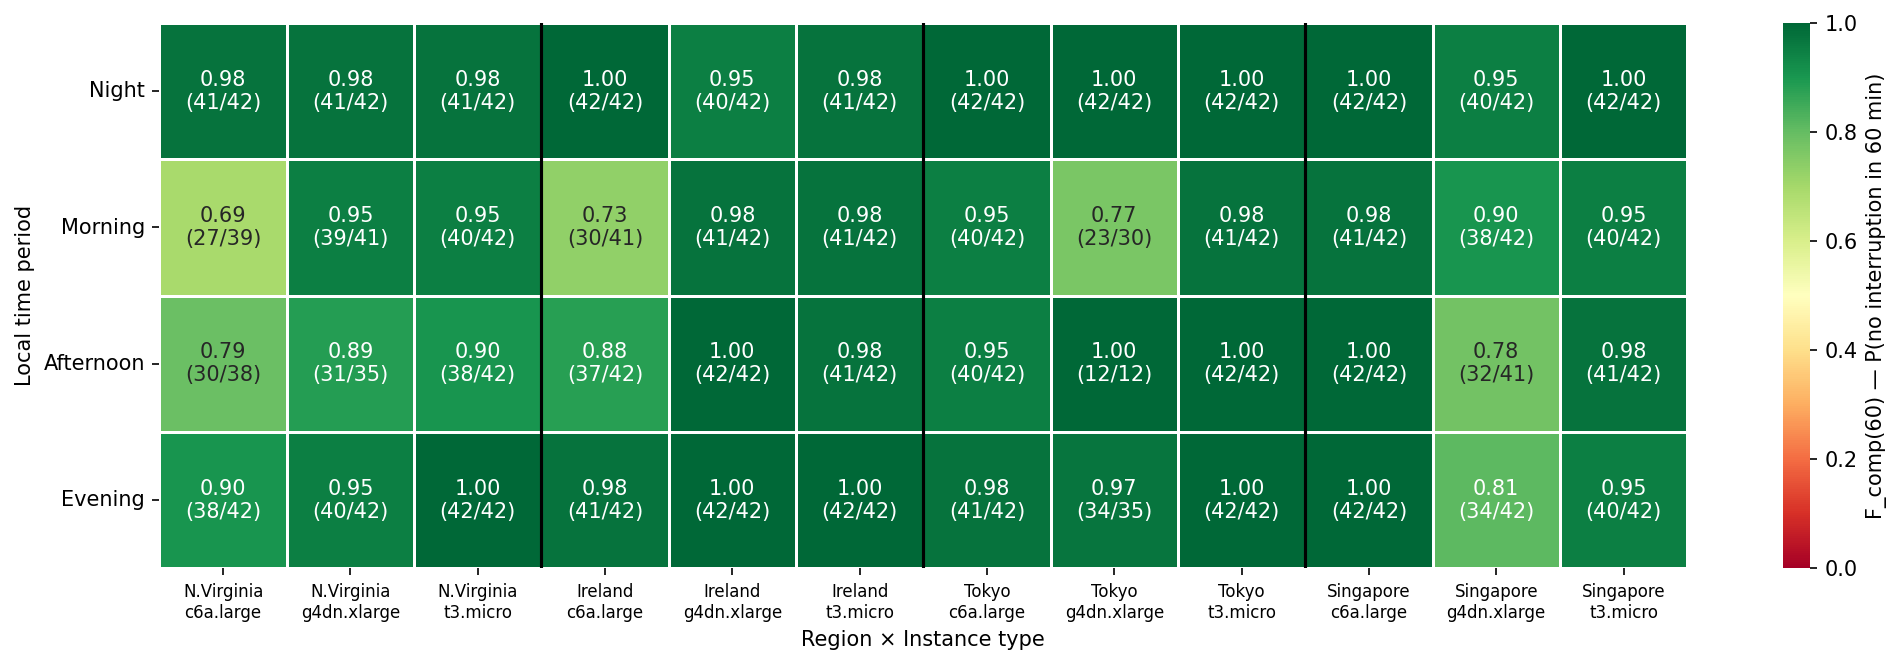
\includegraphics[width=\textwidth]{images/figure1_fcomp60_heatmap.png}
\caption{時間帯，リージョン，インスタンスタイプ別の $\Fcomp(60)$。
注釈は値とサンプル数（$n_{\mathrm{comp}}/n_{\mathrm{succ}}$）を示す。}
\label{fig:heatmap60}
\end{figure}

t3.micro はすべての条件において $\Fcomp(60) \geq 0.95$ を達成しており，
軽量インスタンスは中断に対して比較的頑健であることを示している．
一方 c6a.large および g4dn.xlarge では条件による変動が大きく，
値はおおよそ 0.65 から 1.00 の範囲で変化した．

最大の変動は N.~Virginia の c6a.large において観測された．
時間帯別の値を表~\ref{tab:period_var} に示す．

\begin{table}[htbp]
\centering
\caption{N.~Virginia，c6a.large における時間帯別の $\Fcomp(60)$}
\label{tab:period_var}
\small
\begin{tabular}{@{}lrrr@{}}
\toprule
時間帯 & $\Fcomp(60)$ & 95\% 信頼区間 & $n$ \\
\midrule
Night     & 0.98 & 0.88--1.00 & 42 \\
Morning   & 0.69 & 0.54--0.81 & 39 \\
Afternoon & 0.79 & 0.64--0.89 & 38 \\
Evening   & 0.91 & 0.78--0.96 & 42 \\
\bottomrule
\end{tabular}
\end{table}

Night と Morning の差は約 0.29 であり，
両者の信頼区間は重ならない．
すなわち\textbf{中断されやすさは実行条件によって大きく異なる}．

この変動は，第~\ref{chap:split} 章において
提案手法の効果が条件によってどう変わるかを分析する際の
基礎データとなる．

\subsection{中断ハザード率の挙動}
\label{sec:hazard}

本章の中心的な分析結果を示す．

第~\ref{chap:split} 章の提案は，
\textbf{実行単位を短くすれば中断に遭遇しにくくなる}という前提に立つ．
この前提が成立するかどうかは，
中断ハザード率が経過時間に対してどう振る舞うかに依存する．

もしハザード率が経過時間とともに増加するならば
（すなわち長時間稼働したインスタンスほど中断されやすいならば），
分割の効果は限定的となる．
逆にハザード率が一定であれば，
中断は単位時間あたり一定確率で発生する事象であり，
実行単位を短くすることが直接的に被中断確率の低下につながる．

経過時間区間ごとに，その区間に入る直前まで生存していた
インスタンス数（リスク集合）で正規化したハザード率を
表~\ref{tab:hazard} および図~\ref{fig:hazard} に示す．

\begin{table}[htbp]
\centering
\caption{経過時間別の中断ハザード率（$\Nsucc = 1{,}950$，中断 117 件）}
\label{tab:hazard}
\small
\begin{tabular}{@{}lrrrr@{}}
\toprule
経過時間 & 中断件数 & リスク集合 & 区間あたり & 単位時間あたり \\
\midrule
0--5 分   & 12 & 1,950 & 0.62\% & 0.123 \%/分 \\
5--10 分  & 11 & 1,938 & 0.57\% & 0.114 \%/分 \\
10--20 分 & 25 & 1,927 & 1.30\% & 0.130 \%/分 \\
20--30 分 & 12 & 1,902 & 0.63\% & 0.063 \%/分 \\
30--40 分 & 14 & 1,890 & 0.74\% & 0.074 \%/分 \\
40--50 分 & 23 & 1,876 & 1.23\% & 0.123 \%/分 \\
50--60 分 & 10 & 1,853 & 0.54\% & 0.054 \%/分 \\
\bottomrule
\end{tabular}
\end{table}

\begin{figure}[htbp]
\centering
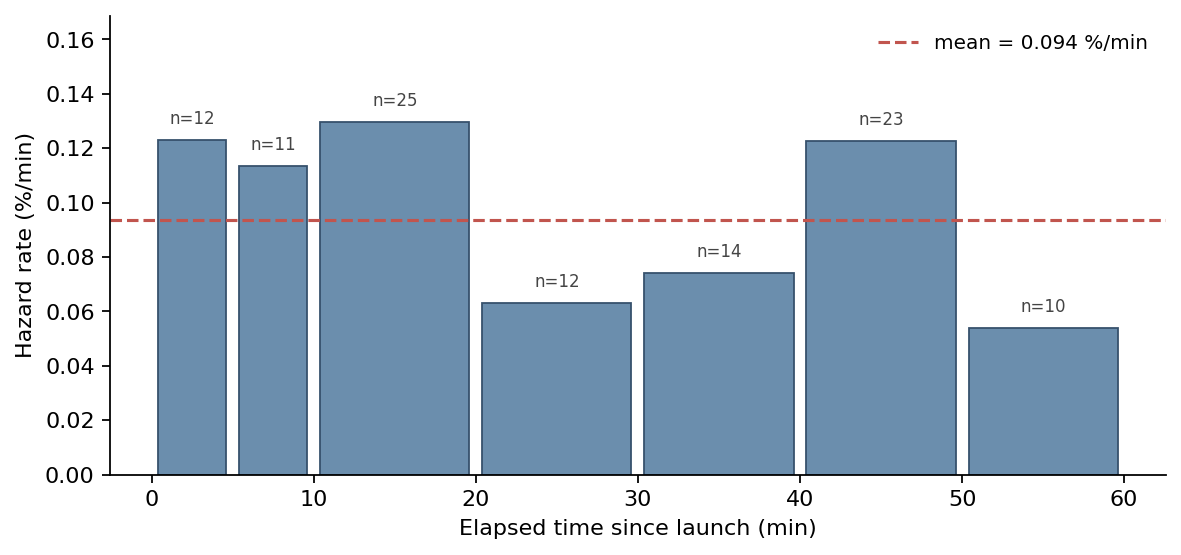
\includegraphics[width=0.85\textwidth]{images/figure3_hazard.png}
\caption{経過時間別の中断ハザード率。単調増加の傾向は見られず，
0.054--0.130 \%/分の範囲で変動する。}
\label{fig:hazard}
\end{figure}

ハザード率は 0.054--0.130 \%/分の範囲で変動するが，
\textbf{経過時間に対する単調増加の傾向は見られない}．
すなわち「長時間稼働したインスタンスほど中断されやすくなる」
という摩耗的な性質は観測されず，
中断は単位時間あたりほぼ一定の確率で発生する
\textbf{近似的にメモリレスな事象}として振る舞う．

\paragraph{この主張の限界．}
中断 117 件という標本数のもとでは，
ハザードの定数性を統計的に強く主張することはできない．
本論文では「単調増加の証拠が得られなかった」という
弱い主張にとどめ，第~\ref{chap:plan} 章の実験で追試する．

\subsection{起動オーバーヘッド}

インスタンスの起動リクエストから実行開始までに要した時間を
表~\ref{tab:startup} に示す．

\begin{table}[htbp]
\centering
\caption{起動オーバーヘッドの実測値（$n = 1{,}950$）}
\label{tab:startup}
\small
\begin{tabular}{@{}lrrrr@{}}
\toprule
 & 平均 & 中央値 & 95 パーセンタイル & 最大 \\
\midrule
起動時間 & 4.52 秒 & 4 秒 & 6 秒 & 30 秒 \\
\bottomrule
\end{tabular}
\end{table}

この値は第~\ref{chap:split} 章のコストモデルにおいて
分割のコストとして用いられる．

\section{本章の限界}
\label{sec:limit_measure}

本章の測定にはいくつかの限界がある．

\begin{itemize}
  \item 観測期間は 1 週間に限定されており，
        各条件のサンプル数は 30--42 である．
        結果は短期的変動を反映している可能性があり，
        長期的・季節的傾向として一般化すべきではない．
  \item 中断されない状態を完了可能性の proxy としており，
        実際のアプリケーションレベルのワークロードは実行していない．
        とりわけ\textbf{チェックポイントのコストは測定していない}．
        この点は第~\ref{chap:split} 章において
        モデルの未確定要素として明示的に扱う．
  \item 各条件につき 1 時間に 1 台のみ起動しているため，
        同時起動の影響やキュー挙動は捉えられていない．
  \item 最大スポット価格を指定していないため，
        デフォルト価格設定下の挙動のみを反映している．
\end{itemize}

\section{本章のまとめ}

本章では測定フレームワークを構築し，
AWS 上で 1 週間の実測を行った．
得られた主要な結果は以下の通りである．

\begin{enumerate}
  \item 起動成功率 $96.7\%$，中断率 $6.0\%$ を観測した．
  \item $\Fcomp(d)$ は期限 $d$ が短いほど高い
        （$d=5$ 分で $0.994$，$d=60$ 分で $0.945$）．
  \item 中断されやすさは実行条件によって大きく異なる
        （N.~Virginia c6a.large で $0.69$--$0.98$）．
  \item \textbf{中断ハザード率は経過時間によらずほぼ一定であり，
        中断は近似的にメモリレスな事象として振る舞う}．
  \item 起動オーバーヘッドは平均 4.52 秒である．
\end{enumerate}

結果 2 と結果 4 は，実行単位を短くすることが
中断対策として有効である可能性を示唆する．
次章ではこれを定量的なモデルとして定式化する．

% =============================================================================
\chapter{分割粒度を考慮した実行モデル}
\label{chap:split}

\section{本章のねらい}

\S\ref{sec:question} で述べたとおり，本論文の問いは
中断による無駄時間の最小化であり，
無駄時間は式~\eqref{eq:intro_waste} の二要素に分解される．

第~\ref{chap:measure} 章の実測により，
この二要素がいずれも\textbf{実行単位の長さ}に依存することが
確認された．

\begin{itemize}
  \item 短い期限ほど $\Fcomp$ が高い（表~\ref{tab:fcomp_overall}）
        \ $\rightarrow$\ 第一要素（やり直す回数）が減る
  \item 中断はメモリレスに発生する（\S\ref{sec:hazard}）
        \ $\rightarrow$\ 短い実行単位ほど損失が小さい，第二要素が減る
\end{itemize}

本章では，ジョブを $k$ 個の断片に分割し
チェックポイントで接続する手法を定式化し，
総無駄時間を最小化する $k$ を求める問題として定式化する．

\paragraph{本章の構成．}
\S\ref{sec:two_effects} で分割が効く理由を整理し，
\S\ref{sec:model} でコストモデルを構築する．
\S\ref{sec:kstar} でこれを実測データに適用して最適分割数を求める．

ただし実際のスポットインスタンスには中断警告の機構が存在し，
これを利用すれば事前の分割を行わずに中断へ対処できる場合がある．
\S\ref{sec:warning} ではこの\textbf{警告駆動復旧}を導入し，
定期分割との比較を通じて
\textbf{いずれの備え方を採用すべきかを決定する枠組み}を示す．
\S\ref{sec:sensitivity} ではチェックポイントコストが
その選択に与える影響を分析し，
\S\ref{sec:condition} でいずれの備えも有効でない場合に頼る
実行条件の選択を検討する．

\section{分割がもたらす二つの効果}
\label{sec:two_effects}

メモリレス性のもとでは，ジョブを分割することにより
二つの効果が同時に働く．

\paragraph{効果 1：断片あたりの被中断確率の低下．}
稼働時間が短いほど中断に遭遇する機会が減る．
第~\ref{chap:measure} 章で測定した $\Fcomp$ がこれに対応する．

\paragraph{効果 2：中断時損失量の低下．}
60 分のジョブが 55 分経過時点で中断されると 55 分が失われるが，
10 分の断片であれば最大 10 分しか失われない
（先行する断片はチェックポイント済みである）．
中断された試行の平均稼働時間
$\bar u(T) = \E[U \mid U < T]$ も，$T$ とともに減少する．

両効果を表~\ref{tab:split_effect} に示す．

\begin{table}[htbp]
\centering
\caption{断片長 $T$ に対する完了確率と中断時平均損失（全データをプール）}
\label{tab:split_effect}
\small
\begin{tabular}{@{}lrrrr@{}}
\toprule
断片長 $T$ & 60 分 & 30 分 & 10 分 & 5 分 \\
\midrule
$\Fcomp(T)$（効果 1） & 0.945 & 0.969 & 0.988 & 0.994 \\
$\bar u(T)$（効果 2） & 26.4 分 & 12.7 分 & 4.9 分 & 2.3 分 \\
\bottomrule
\end{tabular}
\end{table}

これら二つが同時に効くため，分割の効果は非線形に大きい．

\section{コストモデル}
\label{sec:model}

\subsection{記号と決定変数}

ジョブ $j$ は次で特徴づけられる．

\begin{table}[htbp]
\centering
\caption{ジョブの特徴量}
\label{tab:job}
\small
\begin{tabularx}{\textwidth}{@{}llX@{}}
\toprule
記号 & 名称 & 意味 \\
\midrule
$W_j$      & 総計算量 & ジョブ全体の所要時間（分） \\
$k_{\max}$ & 分割上限 & ジョブの性質により定まる分割可能数の上限 \\
\bottomrule
\end{tabularx}
\end{table}

決定変数は\textbf{分割数 $k$} である．
分割数 $k$ のとき，1 断片の長さは $T = W_j / k$ となる．

\subsection{二要素の定量化}

式~\eqref{eq:intro_waste} の二要素を，
第~\ref{chap:measure} 章の実測値を用いて書き下す．

\paragraph{第一要素：やり直す回数．}
断片の完了確率を $p(T)$ とする．
これは第~\ref{chap:measure} 章で定義・測定した
期限条件付き完了可能性そのものである．

\begin{equation}
p(T) \;=\; \Fcomp(T)
\label{eq:p_is_fcomp}
\end{equation}

成功するまで繰り返すときの試行回数は幾何分布に従い，
その期待値は $1/p$ である．
したがってやり直す回数は $1/p - 1$ となる．

\paragraph{第二要素：1 回あたりの損失．}
中断された試行で費やされた時間の期待値を

\begin{equation}
\bar u(T) \;=\; \E\!\left[\,U \;\middle|\; U < T\,\right]
\label{eq:ubar}
\end{equation}

とする．$U$ は観測された稼働時間であり，
第~\ref{chap:measure} 章のデータから直接算出できる．

\subsection{総無駄時間}

断片は $k$ 個あり，各断片について
インスタンスの起動オーバーヘッド $s$ と
チェックポイントコスト $c$ を要する．
したがって総無駄時間は次式で与えられる．

\begin{equation}
\boxed{\;
\Waste(k)
=
\underbrace{k \left( \frac{1}{p(T)} - 1 \right) \bar u(T)}_{\text{やり直し}}
\;+\;
\underbrace{k\,(s + c)}_{\text{起動＋チェックポイント}}
\;,\qquad T = \frac{W_j}{k}
\;}
\label{eq:waste}
\end{equation}

ここで

\begin{itemize}
  \item $s$：インスタンス起動オーバーヘッド。
        第~\ref{chap:measure} 章より\textbf{実測 4.52 秒}
        （表~\ref{tab:startup}）。
  \item $c$：チェックポイントの保存および復元コスト。
        ワークロードの性質に依存するため，
        \textbf{第~\ref{chap:measure} 章の測定からは算出できない}。
        \S\ref{sec:sensitivity} で感度分析を行い，
        第~\ref{chap:plan} 章で実測の計画を示す。
\end{itemize}

第 1 項は $k$ の増加とともに減少し，第 2 項は $k$ に比例して増加する．
したがって $\Waste$ は $k$ に対して U 字型となることが予想される．

\subsection{最適化問題}

以上より，提案手法は次の最適化問題として記述される．

\begin{equation}
\begin{aligned}
\min_{k}\quad
  & \Waste(k) && \text{（総無駄時間）} \\[3pt]
\text{s.t.}\quad
  & k \in \{1, 2, \ldots, k_{\max}\}   && \text{（分割可能性）} \\[2pt]
  & p(W_j/k) \geq p_{\min}             && \text{（信頼性下限）}
\end{aligned}
\label{eq:opt}
\end{equation}

探索空間は $k_{\max}$ 程度と小さく，全列挙により厳密に解ける．

$k = 1$ は分割しない場合に対応し，
従来のスポットインスタンス利用方式に相当する．

\section{最適分割数の存在}
\label{sec:kstar}

式~\eqref{eq:waste} を第~\ref{chap:measure} 章の実測データに適用し，
$k$ に対する総無駄時間を算出した．
推定には Wilson 95\% 下側信頼限界を用い，
標本数が限られることによる楽観的推定を抑制した．

結果を表~\ref{tab:ucurve} に示す（$W_j = 60$ 分，$c = 0$ の場合）．

\begin{table}[htbp]
\centering
\caption{分割数 $k$ に対する総無駄時間（$W_j = 60$ 分，$c = 0$，Wilson LCB）}
\label{tab:ucurve}
\small
\begin{tabular}{@{}rrrrrrr@{}}
\toprule
$k$ & 断片長 & $p_{\mathrm{LCB}}$ & やり直し & 起動 & \textbf{合計} & vs $k{=}1$ \\
\midrule
1  & 60.0 分 & 0.9341 & 1.86 分 & 0.08 分 & \textbf{1.94 分} & --- \\
2  & 30.0 分 & 0.9606 & 1.04 分 & 0.15 分 & \textbf{1.19 分} & $-39\%$ \\
3  & 20.0 分 & 0.9675 & 0.97 分 & 0.23 分 & \textbf{1.19 分} & $-38\%$ \\
4  & 15.0 分 & 0.9728 & 0.91 分 & 0.30 分 & \textbf{1.21 分} & $-38\%$ \\
\textbf{6}  & \textbf{10.0 分} & 0.9824 & 0.53 分 & 0.45 分 & \textbf{0.98 分} & $\mathbf{-50\%}$ \\
10 & 6.0 分  & 0.9880 & 0.34 分 & 0.75 分 & \textbf{1.09 分} & $-44\%$ \\
12 & 5.0 分  & 0.9893 & 0.30 分 & 0.90 分 & \textbf{1.20 分} & $-38\%$ \\
20 & 3.0 分  & 0.9906 & 0.39 分 & 1.51 分 & \textbf{1.90 分} & $-2\%$ \\
60 & 1.0 分  & 0.9980 & 0.00 分 & 4.52 分 & \textbf{4.52 分} & $+133\%$ \\
\bottomrule
\end{tabular}
\end{table}

予想どおり U 字型のカーブが得られた．
$k = 6$（10 分ごとの分割）において総無駄時間は最小となり，
$k=1$ と比較して $50\%$ の削減が得られる．
一方 $k = 60$（1 分ごと）では起動コストが支配的となり，
分割しない場合よりも $133\%$ 悪化する．

すなわち\textbf{「細かく分割するほどよい」という直観は成立せず，
最適分割数 $k^{*}$ が存在する}．

これが本論文の中心的な結果である．

\section{二つの備え方とその選択}
\label{sec:warning}

\subsection{警告駆動復旧}

ここまで，ジョブを事前に $k$ 分割して実行する手法を検討してきた．
しかし実際のスポットインスタンスには，
中断の約 2 分前に警告が通知される機構が存在する~\cite{AWSSpot}．
この警告を利用すれば，\textbf{中断が通知された時点で
はじめてチェックポイントを保存する}という方式が考えられる．
本論文ではこれを\textbf{警告駆動復旧}と呼ぶ．

警告駆動復旧は事前の分割を必要としない．
通常は $k = 1$ のまま実行し，警告を受信した時点で状態を保存して
別のインスタンスで再開する．

両者はコストの支払い方が根本的に異なる．
定期分割が中断の有無にかかわらず $k$ 回のコストを支払うのに対し，
警告駆動復旧は\textbf{中断が実際に発生したときにのみ}支払う．

\begin{table}[htbp]
\centering
\caption{二つの備え方のコスト構造}
\label{tab:two_modes}
\small
\begin{tabularx}{\textwidth}{@{}lXX@{}}
\toprule
 & \textbf{定期分割} & \textbf{警告駆動復旧} \\
\midrule
中断が発生しない場合（$93.4\%$）
  & $k$ 回のコストを支払う
  & 何も支払わない \\
\addlinespace
中断が発生した場合（$6.6\%$）
  & コストに加え，直近の保存地点以降をやり直す
  & 保存が間に合えば損失なし。間に合わなければ全てやり直す \\
\bottomrule
\end{tabularx}
\end{table}

第~\ref{chap:measure} 章で観測された中断率は $6.0\%$ であり，
大部分の実行では中断が発生しない．
したがって両者の優劣は，
\textbf{警告が実際にどの程度機能するか}に依存する．

\subsection{どちらが有利かを決める要因}
\label{sec:which_wins}

警告駆動復旧が成立する場合と，しない場合の双方について，
第~\ref{chap:measure} 章のデータを用いて無駄時間を算出した．
結果を表~\ref{tab:mode_compare} に示す．

\begin{table}[htbp]
\centering
\caption{二つの備え方の無駄時間（$W_j = 60$ 分，Wilson LCB）。
警告駆動復旧の値は，警告が機能し猶予時間内に保存が完了する場合のものである。}
\label{tab:mode_compare}
\small
\begin{tabular}{@{}rrrr@{}}
\toprule
$c$ (秒) & 警告駆動復旧 & 定期分割（最良） & 定期分割の $k^{*}$ \\
\midrule
0   & \textbf{0.00 分} & 0.98 分 & 6 \\
5   & \textbf{0.01 分} & 1.36 分 & 2 \\
10  & \textbf{0.02 分} & 1.52 分 & 2 \\
30  & \textbf{0.04 分} & 2.19 分 & 2 \\
60  & \textbf{0.07 分} & 2.94 分 & 1 \\
120 & 1.94 分 & 3.94 分 & 1 \\
180 & 1.94 分 & 4.94 分 & 1 \\
\bottomrule
\end{tabular}
\end{table}

表~\ref{tab:mode_compare} から二点が読み取れる．

第一に，\textbf{警告が機能し，かつ $c$ が小さい場合，
警告駆動復旧が圧倒的に有利}である．
$c = 30$ 秒でも無駄時間は $0.04$ 分にとどまり，
定期分割の $2.19$ 分を大きく下回る．
中断率が $6.6\%$ と低いため，
平常時にコストを支払わない効果が支配的となる．

第二に，\textbf{$c + s \geq 120$ 秒では警告駆動復旧の利点が消失する}．
猶予時間内に保存が完了しないため，
警告を受信しても全てをやり直すことになり，
無駄時間は無対策の場合と同じ $1.94$ 分となる．

一方で，警告が機能しない場合には評価が逆転する．
警告が通知されない，あるいは猶予が不足する場合，
警告駆動復旧の無駄時間は無対策と同じ $1.94$ 分であるのに対し，
定期分割（$k^{*}=6$，$c=0$）は $0.98$ 分であり，
\textbf{定期分割が有利となる}．

\subsection{選択の基準}
\label{sec:warning_cond}

以上より，いずれの備え方を採用すべきかは
以下の条件によって決まる．

\paragraph{条件 1：猶予時間内に保存と復旧が完了すること．}
警告から終了までの猶予は約 2 分である．
この時間内にチェックポイントの保存と
次のインスタンスの起動を完了しなければならない．すなわち

\begin{equation}
c + s < 120\ \text{秒}
\label{eq:warning_cond}
\end{equation}

が必要である．
第~\ref{chap:measure} 章で実測した $s = 4.52$ 秒は十分小さいため，
実質的には $c$ が条件を決定する．

保存すべき状態が大きいワークロード，
たとえば大規模なモデルパラメータを扱う機械学習の学習処理では，
$c$ が 2 分を超えうる．
この場合，警告を受信しても保存が間に合わない．

\paragraph{条件 2：任意の時点で状態を保存できること．}
警告はジョブの進行と無関係に，任意のタイミングで到着する．
したがって警告駆動復旧は，
\textbf{処理の途中の任意の時点で一貫した状態を切り出せる}ことを要求する．

しかし，この要求を満たさないワークロードが存在する．

\begin{itemize}
  \item 外部システムとのトランザクション処理中であり，
        中間状態が一貫していない場合
  \item 外部 API の呼び出し中であり，
        応答を受け取るまで状態が確定しない場合
  \item 処理の構造上，特定の区切り（反復の境界，
        テストケースの完了時点など）でしか
        状態を保存できない実装となっている場合
\end{itemize}

これらの場合，警告を受信しても直ちには保存できず，
次の保存可能な地点まで処理を進める必要がある．
その地点に到達する前に猶予時間が尽きれば，
作業内容は失われる．

\paragraph{条件 3：警告が十分な確率で通知されること．}
AWS は，2 分の猶予を常に保証するものではないとしている~\cite{AWSSpot}．
ハードウェア障害などに起因する即時終了では，
警告が通知されないか，
通知から終了までの間隔が 2 分に満たない場合がある．

警告が通知されない中断の割合が高ければ，
警告駆動復旧は中断の多くを取り逃がすことになり，
事前の備えである定期分割が有利となる．

第~\ref{chap:measure} 章の測定では警告の受信状況を
記録していないため，その頻度は本論文では定量化できない．
これは第~\ref{chap:plan} 章の測定対象とする．

\subsection{選択の枠組み}
\label{sec:split_role}

以上の三条件により，採用すべき備え方は
表~\ref{tab:strategy_role} のように決定される．

\begin{table}[htbp]
\centering
\caption{条件に応じた備え方の選択}
\label{tab:strategy_role}
\small
\begin{tabularx}{\textwidth}{@{}lXX@{}}
\toprule
条件 & 採用すべき備え方 & 根拠 \\
\midrule
三条件をすべて満たす
  & \textbf{警告駆動復旧}（$k=1$）
  & 中断時のみコストを支払う。
    中断率が低い環境では無駄時間が $0.1$ 分未満に収まる \\
\addlinespace
条件 2 または 3 を満たさない
  & \textbf{定期分割}（$k = k^{*}$）
  & 警告を利用できないため事前の備えが必要。
    粒度は \S\ref{sec:kstar} の方法で決定する \\
\addlinespace
条件 1 を満たさない
  （$c + s \geq 120$ 秒）
  & \textbf{いずれも有効でない}
  & 警告駆動は保存が間に合わず，
    定期分割はコストが利得を上回る（\S\ref{sec:sensitivity}）。
    実行条件の選択（\S\ref{sec:condition}）に頼るほかない \\
\bottomrule
\end{tabularx}
\end{table}

\paragraph{本枠組みの意義．}
ここで重要なのは，\textbf{いずれの条件に該当するかによらず，
本章の枠組みが処方を与える}点である．

スポットインスタンスの利用において，
定期的なチェックポイントの取得は広く推奨されている．
しかし表~\ref{tab:mode_compare} が示すとおり，
警告が機能し $c$ が小さい環境では，
定期的な取得はかえって無駄時間を増加させる．
\textbf{「とりあえず定期的にチェックポイントを取る」という
慣行は，必ずしも最適ではない}．

逆に，警告が十分に機能しない環境や，
任意時点での保存が困難なワークロードでは，
定期分割が唯一の手段となる．
その場合には粒度の設計が問題となり，
\S\ref{sec:kstar} で示した $k^{*}$ の算出が必要となる．

すなわち本章の貢献は，
いずれか一方の手法を推奨することではなく，
\textbf{条件に応じて備え方を選択し，
必要な場合に粒度を決定する枠組みを与える}ことにある．

次節以降では，この枠組みを構成する要素のうち，
\textbf{チェックポイントコスト $c$ が選択に与える影響}
（\S\ref{sec:sensitivity}）と，
\textbf{いずれの備えも有効でない場合に頼る実行条件の選択}
（\S\ref{sec:condition}）を順に検討する．

\section{チェックポイントコストに対する感度}
\label{sec:sensitivity}

表~\ref{tab:ucurve} は $c = 0$，すなわち
チェックポイントが無償であると仮定した理想値である．
実際には状態の保存と復元に時間を要する．

$c$ を変化させたときの総無駄時間と $k^{*}$ を
表~\ref{tab:sensitivity} および図~\ref{fig:ucurve} に示す．

\begin{table}[htbp]
\centering
\caption{チェックポイントコスト $c$ に対する最適分割数 $k^{*}$ の感度。
各セルは総無駄時間（分）を表し，太字は各行の最小値を示す。}
\label{tab:sensitivity}
\small
\begin{tabular}{@{}rrrrrrc@{}}
\toprule
$c$ (秒) & $k{=}1$ & $k{=}2$ & $k{=}4$ & $k{=}6$ & $k{=}12$ & $\mathbf{k^{*}}$ \\
\midrule
0   & 1.94 & 1.19 & 1.21 & \textbf{0.98} & 1.20 & \textbf{6} \\
5   & 2.02 & \textbf{1.36} & 1.54 & 1.48 & 2.20 & \textbf{2} \\
10  & 2.11 & \textbf{1.52} & 1.88 & 1.98 & 3.20 & \textbf{2} \\
30  & 2.44 & \textbf{2.19} & 3.21 & 3.98 & 7.20 & \textbf{2} \\
60  & \textbf{2.94} & 3.19 & 5.21 & 6.98 & 13.20 & \textbf{1} \\
120 & \textbf{3.94} & 5.19 & 9.21 & 12.98 & 25.20 & \textbf{1} \\
\bottomrule
\end{tabular}
\end{table}

\begin{figure}[htbp]
\centering
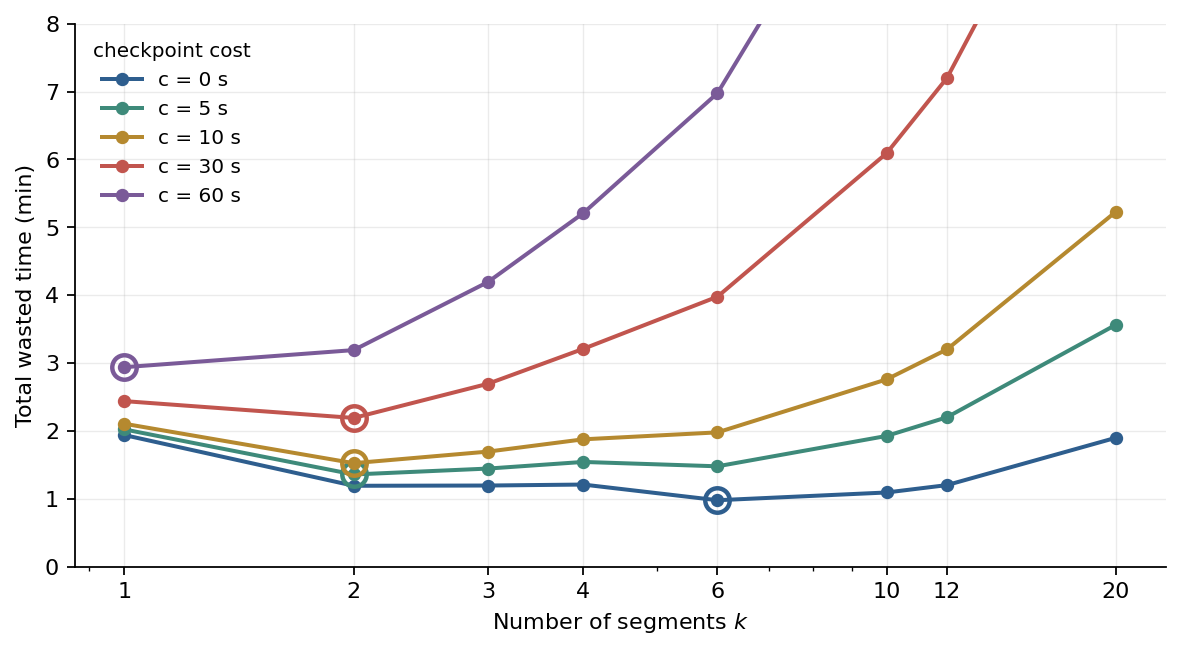
\includegraphics[width=0.9\textwidth]{images/figure4_ucurve.png}
\caption{分割数に対する総無駄時間の U 字カーブ。
各曲線はチェックポイントコスト $c$ の値に対応し，
二重丸は各曲線の最小点 $k^{*}$ を示す。
$c$ の増加とともに $k^{*}$ は左へ移動する。}
\label{fig:ucurve}
\end{figure}

この結果は本研究にとって決定的である．

\begin{itemize}
  \item わずか 5 秒のチェックポイントコストで
        $k^{*}$ は 6 から 2 へ低下する．
  \item $c \geq 60$ 秒では $k^{*} = 1$ となり，
        \textbf{分割そのものが無効}となる．
\end{itemize}

すなわち\textbf{定期分割が有効であるか否かも $c$ の値によって決まる}．

\paragraph{警告駆動復旧との関係．}
ここで \S\ref{sec:warning_cond} の条件 1 と対照すると，
重要な構造が明らかになる．

警告駆動復旧が条件 1 によって利用できなくなるのは
$c + s \geq 120$ 秒のときである．
一方，表~\ref{tab:sensitivity} が示すとおり，
定期分割も $c \geq 60$ 秒で $k^{*} = 1$ となり無効化する．

すなわち\textbf{$c$ が大きい領域では，
警告駆動復旧と定期分割がともに成立しない}．
$c$ を小さくできないワークロードに対しては，
チェックポイントに基づく対策そのものが有効でない．

この関係を表~\ref{tab:c_regime} に整理する．

\begin{table}[htbp]
\centering
\caption{チェックポイントコスト $c$ による対策の選択}
\label{tab:c_regime}
\small
\begin{tabularx}{\textwidth}{@{}llX@{}}
\toprule
$c$ の範囲 & 定期分割の $k^{*}$ & 採用すべき対策 \\
\midrule
$c < 60$ 秒
  & $2$--$6$
  & 任意時点で保存できるなら\textbf{警告駆動復旧}。
    できないなら\textbf{定期分割}（$k = k^{*}$） \\
\addlinespace
$60 \leq c < 120$ 秒
  & $1$（無効）
  & 任意時点で保存できるなら\textbf{警告駆動復旧}。
    できないなら\textbf{打つ手がない} \\
\addlinespace
$c \geq 120$ 秒
  & $1$（無効）
  & \textbf{いずれも成立しない}。
    実行条件の選択（\S\ref{sec:condition}）に頼るほかない \\
\bottomrule
\end{tabularx}
\end{table}

\paragraph{実務上の含意．}
以上より，実装上の指針は次のように整理される．

\begin{enumerate}
  \item \textbf{まず $c$ を小さくすることを試みる}．
        増分チェックポイント，保存対象の絞り込み，
        ローカルストレージの活用などにより $c$ を削減できれば，
        警告駆動復旧が利用可能となり，
        平常時のコストを支払わずに中断に対処できる．
  \item 任意時点での保存が実装上困難な場合に限り，
        \textbf{定期分割を採用し，$c$ の実測値に基づいて
        $k^{*}$ を決定する}．
  \item いずれも成立しない場合は，
        中断されにくい実行条件を選択する以外に手段がない．
\end{enumerate}

とりわけ指針 2 について，
\textbf{「とりあえず細かくチェックポイントを取る」
という実装方針は最適ではない}．
表~\ref{tab:sensitivity} が示すとおり，
$c = 30$ 秒のワークロードで $k = 12$ と細分化すると，
無駄時間は $k^{*} = 2$ の場合の $3$ 倍以上に達する．

\section{条件による効果の違い}
\label{sec:condition}

第~\ref{chap:measure} 章で観測したとおり，
中断されやすさは実行条件によって大きく異なる
（表~\ref{tab:period_var}）．
そこで，条件ごとに提案手法の効果がどう変わるかを分析した．

時間帯ごとの総無駄時間を
表~\ref{tab:period_k} および図~\ref{fig:period_k} に示す．

\begin{table}[htbp]
\centering
\caption{時間帯ごとの総無駄時間（分，$W_j = 60$ 分，$c=0$，Wilson LCB）。
太字は各行の最小値を示す。}
\label{tab:period_k}
\small
\begin{tabular}{@{}lrrrrrrrcr@{}}
\toprule
時間帯 & $k{=}1$ & $k{=}2$ & $k{=}3$ & $k{=}4$ & $k{=}6$ & $k{=}10$ & $k{=}12$
 & $\mathbf{k^{*}}$ & 削減 \\
\midrule
Night     & 1.09 & 0.73 & \textbf{0.30} & 0.40 & 0.60 & 0.99 & 1.19
 & \textbf{3}  & $-73\%$ \\
Morning   & 3.81 & 2.13 & 1.99 & 2.07 & \textbf{1.62} & 1.85 & 1.72
 & \textbf{6}  & $-58\%$ \\
Afternoon & 2.58 & 2.18 & 2.34 & 2.06 & 1.69 & \textbf{1.27} & 1.52
 & \textbf{10} & $-51\%$ \\
Evening   & 2.05 & 1.00 & 1.29 & 1.51 & 1.06 & \textbf{0.75} & 0.90
 & \textbf{10} & $-63\%$ \\
\bottomrule
\end{tabular}
\end{table}

\begin{figure}[htbp]
\centering
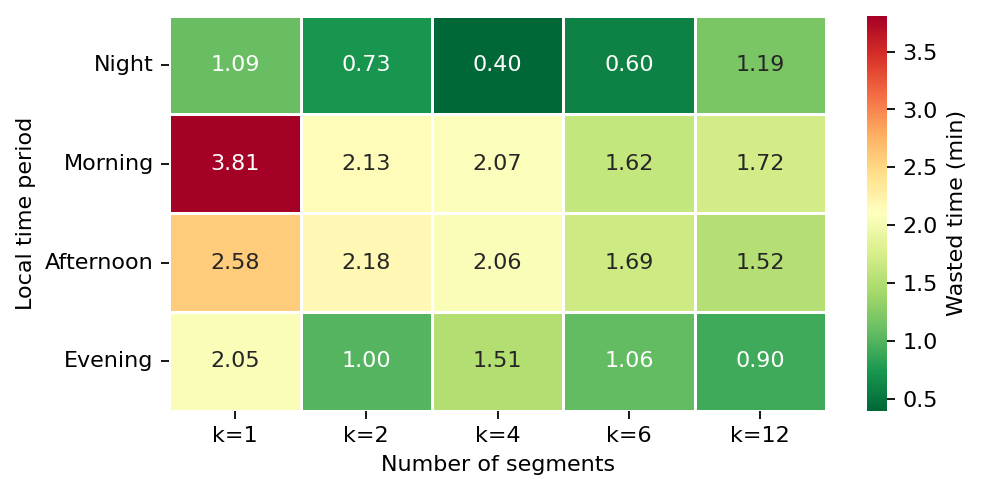
\includegraphics[width=0.75\textwidth]{images/figure5_period_k.png}
\caption{時間帯と分割数の組み合わせによる総無駄時間。
色が濃いほど無駄時間が大きい。}
\label{fig:period_k}
\end{figure}

表~\ref{tab:period_k} から次の三点が読み取れる．

\begin{enumerate}
  \item \textbf{すべての条件で分割は有効である}．
        削減率は $51\%$--$73\%$ であり，
        いずれの時間帯においても $k^{*} > 1$ となる．
  \item \textbf{最適分割数は条件によって異なる}．
        $k^{*}$ は 3 から 10 まで変動する．
        したがって\textbf{単一の推奨粒度を与えることはできず，
        対象環境の中断特性に基づいて決定する必要がある}．
  \item 最も中断されやすい条件（Morning，$k{=}1$）の 3.81 分は，
        分割により 1.62 分まで低下する．
        これは最も中断されにくい条件（Night，$k{=}1$）の 1.09 分に
        近い水準であり，
        \textbf{分割によって実行条件の不利をある程度補償できる}
        ことを示す．
\end{enumerate}

結果 2 は本手法の設計指針に関わる．
最適粒度が条件に依存する以上，
提案手法の価値は「10 分ごとに切れ」といった固定的な推奨ではなく，
\textbf{測定値から $k^{*}$ を算出する枠組みを与える}点にある．

結果 3 は実務上重要である．
実行条件を選べない場合，すなわち即時実行が要求される場合でも，
分割によって中断リスクを低減できることを意味する．

\paragraph{注意．}
表~\ref{tab:period_k} の値は時間帯ごとに層別しているため，
各セルの標本数は全体の約 1/4（約 490 件）に減少する．
とりわけ Night 期間は中断件数が少なく，
$k^{*}=3$ という値は標本変動の影響を受けている可能性がある．
時間帯別の $k^{*}$ は参考値として扱い，
全データをプールした \S\ref{sec:kstar} の結果を主結果とする．

\section{本章のまとめ}

本章では，分割粒度 $k$ を決定変数とするコストモデルを構築し，
第~\ref{chap:measure} 章の実測データに適用した．

得られた主要な結果は以下の通りである．

\begin{enumerate}
  \item 中断への備え方には\textbf{警告駆動復旧}と\textbf{定期分割}の
        二つがあり，両者はコストの支払い方が異なる．
        前者は中断時にのみ，後者は中断の有無によらず支払う．
  \item いずれを採用すべきかは\textbf{三つの条件}によって決まる．
        猶予時間内に保存と復旧が完了すること（$c + s < 120$ 秒），
        任意の時点で一貫した状態を保存できること，
        警告が十分な確率で通知されることである（\S\ref{sec:warning}）．
        観測された中断率 $6.0\%$ のもとでは，
        三条件を満たす場合に警告駆動復旧が有利であり
        （無駄時間 $0.1$ 分未満），
        満たさない場合には定期分割が有利となる．
  \item 定期分割が必要となった場合，総無駄時間は $k$ に対して U 字型となり，
        \textbf{最適分割数 $k^{*}$ が存在する}．
        $c=0$ のとき $k^{*}=6$ であり，$k=1$ と比べ $50\%$ の削減となる．
        「細かく分割するほどよい」という実装方針は最適ではない．
  \item $k^{*}$ は\textbf{チェックポイントコスト $c$ に支配される}．
        $c=5$ 秒で $k^{*}=2$，$c \geq 60$ 秒で $k^{*}=1$ となる．
        $c$ が大きい領域では警告駆動復旧と定期分割がともに成立せず，
        実行条件の選択に頼るほかない．
  \item 実行条件を層別すると $k^{*}$ は 3 から 10 まで変動する．
        したがって固定的な推奨粒度ではなく，
        測定値から $k^{*}$ を算出する枠組みが必要である．
\end{enumerate}

本章が与えるのは，いずれか一方の手法の推奨ではなく，
\textbf{条件に応じて備え方を選択し，
必要な場合に粒度を決定する枠組み}である．
枠組みのどの分岐に該当するかは，
チェックポイントコスト $c$ と警告の受信状況によって決まるが，
いずれも第~\ref{chap:measure} 章の測定では取得していない．
次章では，これらを解消する検証計画を示す．

% =============================================================================
\chapter{検証計画}
\label{chap:plan}

\section{検証すべき事項}

\S\ref{sec:sensitivity} で示したとおり，
第~\ref{chap:split} 章のモデルには未確定要素が一つある．
チェックポイントコスト $c$ である．

$c$ の値によって $k^{*}$ は 6 から 1 まで変化し，
$c \geq 60$ 秒では提案手法そのものが無効となる．
起動オーバーヘッド $s$ が第~\ref{chap:measure} 章の測定から
実測できたのに対し，
$c$ はワークロードの性質に依存するため，
既存データからは算出できない．

したがって検証の目的を以下の優先順位で設定する．

\begin{table}[htbp]
\centering
\caption{検証の目的と優先順位}
\label{tab:objectives}
\small
\begin{tabularx}{\textwidth}{@{}clX@{}}
\toprule
優先 & 目的 & 理由 \\
\midrule
1 & \textbf{$c$ の実測}
  & 警告駆動復旧が成立するか（$c+s<120$ 秒）と，
    成立しない場合の $k^{*}$ の双方を決定する \\
\addlinespace
1' & \textbf{警告の受信状況の測定}
  & 警告駆動復旧の前提。中断時に警告が通知されたか，
    通知から終了までの猶予が実際にどれだけかは未測定 \\
\addlinespace
2 & U 字カーブの検証
  & 式~\eqref{eq:waste} の妥当性検証 \\
\addlinespace
3 & 中断の独立性の検証
  & 期待試行回数 $1/p$ の前提の検証 \\
\addlinespace
4 & メモリレス性の追試
  & \S\ref{sec:hazard} の前提の検証 \\
\bottomrule
\end{tabularx}
\end{table}

\section{対象ワークロードの選定}

\subsection{選定基準}

\begin{itemize}
  \item 実行時間が 30 分以上であること
        （短いと $\Fcomp > 0.99$ となり差が検出できない）
  \item チェックポイントが実装可能であること
  \item $c$ が現実的に測定できること
  \item 中断率の高い条件を選択できること
\end{itemize}

\subsection{候補の比較}

\S\ref{sec:sensitivity} の分析は，$c$ の大きさによって
結論が変わることを示した．
したがって\textbf{$c$ が対照的な二つのワークロード}を
選定することが望ましい．

\begin{table}[htbp]
\centering
\caption{対象ワークロードの候補}
\label{tab:usecases}
\small
\begin{tabularx}{\textwidth}{@{}lXX@{}}
\toprule
 & \textbf{A: 機械学習の学習} & \textbf{B: CI/CD テスト} \\
\midrule
分割の単位   & エポック & テストシャード \\
チェックポイント & モデルパラメータの保存・復元 & 結果記録の保存 \\
想定 $c$     & \textbf{30--120 秒}（数百 MB） & \textbf{1--5 秒}（数 KB） \\
予測 $k^{*}$ & \textbf{1--2（分割は無効）} & \textbf{2--6（分割が有効）} \\
インスタンス & g4dn.xlarge & c6a.large \\
中断率       & 高い & 低い \\
\bottomrule
\end{tabularx}
\end{table}

両者を実施することで，
\textbf{どのようなワークロードであれば分割が有効か}という
一般的な指針が得られる．
これは単一ワークロードによる評価よりも強い主張となる．

一方のみを実施する場合は B（CI/CD テスト）を選択する．
コストが約 1/10 であり，$c$ が小さく
分割が有効となる可能性が高いためである．

\section{実験 1：チェックポイントコストの実測}

\paragraph{目的．}
$c$ を実測し，図~\ref{fig:ucurve} の理論曲線上で
$k^{*}$ を確定する．

\paragraph{方法．}
中断のない環境において分割数 $k$ を変化させ，
純粋なオーバーヘッドのみを測定する．
各断片についてチェックポイントの保存時間，
復元時間，インスタンス起動時間を記録し，
$c = \text{保存} + \text{復元}$ の平均を求める．

\paragraph{規模．}
$k \in \{1,2,4,6,12\}$ をそれぞれ 10 回実施する．
断片数の合計は $(1+2+4+6+12)\times 10 = 250$ 本，
総計算時間は約 50 時間である．
中断の発生を待つ必要がないため \textbf{1--2 日で完了}する．
コストは c6a.large で約 \$1.5 である．

\paragraph{意義．}
この実験の結果のみで，理論曲線上の $k^{*}$ が確定する．
以降の実験設計はこの結果を踏まえて確定させる．

\section{実験 2：U 字カーブの検証}

\paragraph{目的．}
実測された $c$ のもとで予測される $k^{*}$ が，
実際に総無駄時間を最小化するかを検証する．

\paragraph{方法．}
中断が発生しやすい条件として
N.~Virginia，c6a.large，Morning 期間を選択する
（第~\ref{chap:measure} 章において $\Fcomp(60) = 0.69$ と最低値を記録）．
$k \in \{1,2,4,6,12\}$ を各 24 回／日，14 日間実施する．
中断された場合は当該断片のみを再実行し，
先行する断片はチェックポイントから復元する．

\paragraph{測定項目．}
総課金時間，やり直し回数，完了までの実時間．

\paragraph{規模．}
$5 \times 24 \times 14 = 1{,}680$ 本の実行．
コストは約 \$25 である．

\section{実験 3：中断の独立性の検証}

\paragraph{目的．}
「中断された直後の再試行も同じ確率 $p$ で成功する」
という仮定を検証する．

式~\eqref{eq:waste} における期待試行回数 $1/p$ は，
各試行が独立であることを前提としている．
しかし中断は容量逼迫時に発生すると考えられるため，
直後の再試行はより失敗しやすい可能性がある．
その場合 $p$ は過大評価であり，
分割の効果も割り引いて解釈する必要がある．

\paragraph{方法．}
中断を検知した場合に即座に同一条件で再起動し，
2 回目の成否を記録する．
1 回目の $p$ と 2 回目の $p$ を比較する．

\paragraph{規模．}
中断 50 件の収集を目標とする．
中断率 6\% のもとでは約 830 回の起動を要する．
\textbf{実験 2 と同一の実行に相乗りできる}
（実験 2 で中断された断片の再試行結果を記録すればよい）．

\section{実験規模のまとめ}

\begin{table}[htbp]
\centering
\caption{検証実験の規模とコスト（c6a.large を想定）}
\label{tab:exp_scale}
\small
\begin{tabularx}{\textwidth}{@{}llrX@{}}
\toprule
実験 & 期間 & コスト & 得られるもの \\
\midrule
1: $c$ の実測   & \textbf{1--2 日} & \$1.5 & \textbf{$k^{*}$ の確定} \\
2: U 字検証     & 2 週間 & \$25 & モデルの妥当性 \\
3: 独立性       & 実験 2 に相乗り & \$0 & 前提の検証 \\
\midrule
\textbf{合計}   & \textbf{約 3 週間} & \textbf{約 \$27} & \\
\bottomrule
\end{tabularx}
\end{table}

機械学習ワークロード（実験 1 のみ g4dn.xlarge で追加実施）を
含めても約 \$40 である．

\section{実装方針}

第~\ref{chap:measure} 章で構築した測定フレームワークを流用する．
変更点を表~\ref{tab:impl} に示す．

\begin{table}[htbp]
\centering
\caption{既存実装からの変更点}
\label{tab:impl}
\small
\begin{tabularx}{\textwidth}{@{}lX@{}}
\toprule
既存要素 & 変更内容 \\
\midrule
起動処理 & 待機処理を実ワークロードに置換 \\
中断検知 & そのまま流用（インスタンスメタデータの監視） \\
記録項目 & 断片番号，分割数，保存時間，復元時間を追加 \\
スケジューラ & 「断片完了後に次の断片を起動」する連鎖を追加 \\
\bottomrule
\end{tabularx}
\end{table}

チェックポイントの保存先はオブジェクトストレージとし，
各断片は直前の断片が保存した状態を読み込み，
処理後に次の状態を書き出す．

\section{測定結果と結論の対応}
\label{sec:outcome_map}

\S\ref{sec:split_role} で示した枠組みは，
測定結果がいずれであっても処方を与える．
その対応を表~\ref{tab:outcome_map} に示す．

\begin{table}[htbp]
\centering
\caption{測定結果と導かれる結論の対応}
\label{tab:outcome_map}
\small
\begin{tabularx}{\textwidth}{@{}llX@{}}
\toprule
警告の受信状況 & $c$ の実測値 & 導かれる結論 \\
\midrule
十分に機能する & $c + s < 120$ 秒
  & \textbf{事前の分割は不要}。警告駆動復旧で足りる。
    定期的なチェックポイント取得という慣行は
    かえって無駄時間を増加させる \\
\addlinespace
十分に機能する & $c + s \geq 120$ 秒
  & いずれの備えも有効でない。
    $c$ の削減を図るか，実行条件の選択に頼る \\
\addlinespace
機能しない & 任意
  & \textbf{事前分割が必要}。
    粒度は \S\ref{sec:kstar} の方法により $k^{*}$ として決定する \\
\bottomrule
\end{tabularx}
\end{table}

いずれの行に該当するかは測定によって決まるが，
\textbf{どの行であっても実務上の処方が得られる}点が重要である．
本研究の貢献は特定の手法の推奨ではなく，
この対応関係そのものにある．

\section{事前分割を選ぶ場合の粒度}

表~\ref{tab:outcome_map} の第三行，
すなわち事前分割を採用すべきと判定された場合について，
実験 1 で得られる $c$ の値に応じた粒度を表~\ref{tab:outcomes} に示す．

\begin{table}[htbp]
\centering
\caption{チェックポイントコストの実測値に応じた結論}
\label{tab:outcomes}
\small
\begin{tabularx}{\textwidth}{@{}llX@{}}
\toprule
$c$ の実測値 & $k^{*}$ & 導かれる結論 \\
\midrule
$c < 5$ 秒 & 4--6
  & 分割は有効であり，最適粒度は約 10 分 \\
\addlinespace
$5 \leq c < 30$ 秒 & 2
  & 分割は有効だが粗く切るべきであり，細分化は逆効果 \\
\addlinespace
$30 \leq c < 60$ 秒 & 2
  & 分割による利得は限定的 \\
\addlinespace
$c \geq 60$ 秒 & 1
  & \textbf{当該ワークロードでは分割は成立しない。
    状態の大きいワークロードには別の中断対策が必要である} \\
\bottomrule
\end{tabularx}
\end{table}

\section{リスクと対策}

\begin{table}[htbp]
\centering
\caption{想定されるリスクと対策}
\label{tab:risks}
\small
\begin{tabularx}{\textwidth}{@{}XXX@{}}
\toprule
リスク & 影響 & 対策 \\
\midrule
$c$ が大きく分割が無効
  & 提案の前提が崩れる
  & 実験 1 を最優先し 1--2 日で判明させる。
    無効でも適用条件を示す結果として報告する \\
\addlinespace
中断が十分に集まらない
  & 実験 2 の検出力不足
  & 中断率が最も高い条件に集中させる \\
\addlinespace
メモリレス性が成立しない
  & 分割の前提が崩れる
  & 実験で追試する。標本数 117 の限界を明記済み
    （\S\ref{sec:hazard}） \\
\addlinespace
独立性が成立しない
  & $p$ が過大評価となる
  & 実験 3 で検証し，必要なら条件付き確率へ修正する \\
\addlinespace
観測期間と実験期間の市場変化
  & 予測が外れる
  & 実験期間中に $\Fcomp$ を再測定し比較する \\
\bottomrule
\end{tabularx}
\end{table}

% =============================================================================
\chapter{結論}
\label{chap:conclusion}

\section{本論文のまとめ}

本論文は，\textbf{中断によって失われる時間を最小化するには
ジョブをどのような単位で実行すればよいか}という問いに取り組んだ．

この無駄時間が\textbf{やり直す回数}と\textbf{1 回あたりの損失}の
積に分解され（式~\eqref{eq:intro_waste}），
両者がいずれも実行単位の長さに依存することに着目し，
\textbf{分割粒度}を設計変数とする手法を提案した．

第~\ref{chap:measure} 章では，スポットインスタンスの信頼性を
期限条件付き完了可能性 $\Fcomp(d)$ として定義し，
測定フレームワークを実装して
AWS 上で 1 週間の実測（$\Nreq = 2{,}016$）を行った．
その結果，起動成功率 $96.7\%$，中断率 $6.0\%$ を観測するとともに，
\textbf{中断ハザード率が経過時間によらずほぼ一定}であり，
中断が近似的にメモリレスな事象として振る舞うことを示した．

第~\ref{chap:split} 章では，中断への備え方を
\textbf{事前分割}と\textbf{警告駆動復旧}の二つに整理し，
同一のコストモデル上で比較した．
中断は大部分の実行では発生しない（観測された中断率は $6.0\%$）ため，
中断時にのみコストを支払う警告駆動復旧が有利となりうる．
その成立条件を三点として定式化し，
条件を満たす場合には無駄時間が $0.1$ 分未満にとどまり
\textbf{事前の分割が不要である}ことを示した．
これは，定期的なチェックポイント取得という広く行われている慣行が
必ずしも最適でないことを意味する．

一方，条件を満たさない場合の手段として，
分割粒度 $k$ を決定変数とするコストモデルを構築した．
実測データへの適用により，
総無駄時間が $k$ に対して U 字型となること，
すなわち\textbf{最適分割数 $k^{*}$ が存在する}ことを示した．
$c = 0$ のとき $k^{*} = 6$ であり，分割しない場合と比べて
$50\%$ の削減が得られる．

さらに感度分析により，$k^{*}$ が
\textbf{チェックポイントコスト $c$ に支配される}ことを明らかにした．
$c = 5$ 秒で $k^{*}$ は 2 に低下し，
$c \geq 60$ 秒では分割そのものが無効となる．
$c$ が大きい領域では警告駆動復旧と定期分割がともに成立せず，
実行条件の選択に頼るほかないことも示された．

第~\ref{chap:plan} 章では，未確定要素である $c$ の実測を
最優先とする検証計画を示した．

\section{本研究の意義}

本研究の意義は以下の四点である．

\begin{enumerate}
  \item スポットインスタンスの信頼性を，
        プロバイダ固有の不透明な指標ではなく，
        直接観測された起動・中断記録のみから算出される
        \textbf{解釈可能な指標}として定式化した．
  \item 中断への二つの備え方を同一のモデル上で比較し，
        \textbf{条件に応じて選択する枠組み}を与えた．
        この枠組みは，警告が機能する環境では「備えは不要」，
        機能しない環境では「粒度 $k^{*}$ で分割せよ」という
        異なる処方を，同一の基準から導く．
  \item 従来は実装の都合で決められてきた\textbf{チェックポイント間隔}を，
        中断特性に基づく\textbf{最適化問題}として定式化した．
  \item 「細かく分割するほどよい」という直観に反し，
        \textbf{最適分割数が存在し，それがチェックポイントコストに
        支配される}ことを定量的に示した．
        これは実務者に対し，
        分割粒度を測定に基づいて決定すべきであるという
        具体的な指針を与える．
\end{enumerate}

\section{今後の課題}

\begin{itemize}
  \item 第~\ref{chap:plan} 章の検証計画の実施，
        とりわけチェックポイントコスト $c$ の実測
  \item 観測期間の延長による，季節変動を含む長期的傾向の把握
  \item 中断のメモリレス性に関する，より大きな標本に基づく検証
  \item 分割不可能なワークロードに対する代替手法の検討
  \item 実際の CI/CD ワークロードおよび機械学習ワークロードにおける評価
\end{itemize}

% =============================================================================
\chapter*{謝辞}
\addcontentsline{toc}{chapter}{謝辞}

本研究を進めるにあたり，終始丁寧なご指導を賜りました
指導教員の先生方に深く感謝いたします．
また，日頃より有益な議論をいただいた研究室の皆様に御礼申し上げます．

% =============================================================================
\begin{thebibliography}{99}
\addcontentsline{toc}{chapter}{参考文献}

\bibitem{AWSSpot}
Amazon Web Services:
Amazon EC2 Spot Instances.
\url{https://aws.amazon.com/ec2/spot/}
(Accessed: May 2026)

\bibitem{Lin2022Survey}
Lin, L., Pan, L., Liu, S.:
Methods for improving the availability of spot instances: A survey.
Computers in Industry, 141, 103718 (2022).

\bibitem{Ramesh2025}
Ramesh, D.G.A., Lennon, R.G.:
Evaluating the Impact of Reserved Instances vs. Spot Instances in DevOps Cloud Workflows.
In: 2025 35th Irish Signals and Systems Conference (ISSC). IEEE (2025).

\bibitem{Garg2025}
Garg, D., Kaata, S.K., Bhumireddy, D.R., Bolla, B.K.:
Reducing Cloud Cost Through Optimized Bidding for AWS Spot Instances.
In: 2025 3rd International Conference on Advances in Computation,
Communication and Information Technology (ICAICCIT). IEEE (2025).

\bibitem{Katayama2022}
Katayama, D., Kasai, K., Koita, T.:
Migration Destination Selection Algorithm for Spot Instances using SPS.
In: 2022 IEEE International Conference on Big Data (Big Data),
pp. 6690--6692. IEEE, Osaka (2022).

\bibitem{Kim2024SpotInterruption}
Kim, K., Lee, K.:
Making Cloud Spot Instance Interruption Events Visible.
In: Proceedings of the ACM Web Conference 2024 (WWW '24),
pp. 2998--3009. ACM, New York (2024).

\bibitem{AWSSPS}
Amazon Web Services:
Spot Placement Score. Amazon EC2 User Guide.
\url{https://docs.aws.amazon.com/AWSEC2/latest/UserGuide/spot-placement-score.html}
(Accessed: May 2026)

\bibitem{Lee2022SpotLake}
Lee, S., Hwang, J., Lee, K.:
SpotLake: Diverse Spot Instance Dataset Archive Service.
In: 2022 IEEE International Symposium on Workload Characterization (IISWC),
pp. 242--255. IEEE (2022).

\bibitem{Pham2018}
Pham, T.-P., Ristov, S., Fahringer, T.:
Performance and Behavior Characterization of Amazon EC2 Spot Instances.
In: 2018 IEEE 11th International Conference on Cloud Computing (CLOUD).
IEEE (2018).

\bibitem{AWSInstanceTypes}
Amazon Web Services:
Amazon EC2 Instance Types. Amazon EC2 User Guide.
\url{https://docs.aws.amazon.com/AWSEC2/latest/UserGuide/instance-types.html}
(Accessed: May 2026)

\end{thebibliography}

\end{document}
